
%(BEGIN_QUESTION)
% Copyright 2007, Tony R. Kuphaldt, released under the Creative Commons Attribution License (v 1.0)
% This means you may do almost anything with this work of mine, so long as you give me proper credit

The amount of energy stored in an electrical capacitor is given by the following formula:

$$U = {1 \over 2}CV^2$$

\noindent
Where,

$U$ = Potential energy, in Joules (J)

$C$ = Capacitance, in Farads (F)

$V$ = Voltage across capacitor terminals, in volts (V)

\vskip 30pt

Similarly, the amount of energy stored in an electrical inductor is given by the following formula:

$$U = {1 \over 2}LI^2$$

\noindent
Where,

$U$ = Potential energy, in Joules (J)

$L$ = Inductance, in Henrys (H)

$I$ = Current through inductor coil, in amperes (A)

\vskip 30pt

A very early standard for analog instrumentation signals was 10 to 50 milliamps DC, in contrast to the more modern analog standard of 4 to 20 milliamps DC.  Calculate how much more energy would be stored by a given inductance inside a 10-50 mA field instrument versus a 4-20 mA field instrument, at the same percentage of signal range.  In other words, calculate the {\it ratio} of energy stored from the old instrument to the new instrument under equivalent operating conditions.

$$\includegraphics[width=15.5cm]{i02466x01.eps}$$

\vskip 10pt

\filbreak

Older 10-50 mA instrument loops commonly used 90 volt DC power supplies, instead of the 24 volt DC power supplies typically used to power modern 4-20 mA loop-powered instruments.  Calculate how much more energy would be stored by a given capacitance inside a 10-50 mA field instrument versus a 4-20 mA field instrument, at maximum terminal voltage.  In other words, calculate the {\it ratio} of energy stored from the old instrument to the new instrument under equivalent operating conditions.

$$\includegraphics[width=15.5cm]{i02466x02.eps}$$

\vskip 20pt \vbox{\hrule \hbox{\strut \vrule{} {\bf Suggestions for Socratic discussion} \vrule} \hrule}

\begin{itemize}
\item{} Explain why the 10-50 mA signal standard was once widely used in industrial control systems.  Why didn't a lower-value current standard such as 4-20 mA gain acceptance initially, especially when you consider that the power supplies used with most 10-50 mA transmitters were of a high enough voltage to pose a shock hazard?
\end{itemize}

\underbar{file i02466}
%(END_QUESTION)





%(BEGIN_ANSWER)

Energy ratio from perspective of voltage = $\left({90 \over 24}\right)^2$ = 14.0625:1.

\vskip 10pt

Energy ratio from perspective of current = $\left({50 \over 20}\right)^2$ = 6.25:1.

\vskip 10pt

I find it fascinating how the physics of electricity so closely parallels the physics of Newtonian mechanics.  Note how both formulae for energy closely resemble the formula for kinetic energy of a moving object:

$$E_k = {1 \over 2}mv^2$$

\vskip 10pt

Inductors store energy in the form of a magnetic field, and magnetic fields are directly proportional in strength to the amount of current going through a conductor.  Current ($I$) in this case is analogous to the velocity ($v$) of a mass, and inductance ($L$) is analogous to the mass itself ($m$), making stored energy proportional to $LI^2$.

\vskip 10pt

Capacitors store energy in the form of an electric field, and electric fields are directly proportional in strength to the amount of voltage existing between two conductors.  Voltage ($V$) in this case is analogous to the velocity ($v$) of a mass, and capacitance ($C$) is analogous to the mass itself ($m$), making stored energy proportional to $CV^2$.


%(END_ANSWER)





%(BEGIN_NOTES)

\vfil \eject

\noindent
{\bf Summary Quiz:}

Suppose a capacitor stores 290 millijoules of energy at a steady voltage of 13.2 volts.  If the voltage is increased to 26.4 volts, the energy stored by this same capacitor will be:

\begin{itemize}
\item{} 145 millijoules
\vskip 5pt 
\item{} 5 millijoules
\vskip 5pt 
\item{} 290 millijoules
\vskip 5pt 
\item{} 72.5 millijoules
\vskip 5pt 
\item{} 580 millijoules
\vskip 5pt 
\item{} 1160 millijoules
\end{itemize}


%INDEX% Electronics review: energy stored in a capacitor
%INDEX% Electronics review: energy stored in an inductor

%(END_NOTES)


